% !TeX spellcheck = ru_RU
% !TeX root = lambda2023.tex

\begin{frame}{Состояние математики в 1910-х}

 	Матан, алгебра, геометрия...\\
 	Информатики (computer science) явным образом пока нет, как часть математики\\

 	Математическая логика
 	\begin{enumerate}
 		\item Пытается формализовать интуитивно понятные утверждения
 		\item Языки (т.е. синтаксис), чтобы на них можно было правильно сформулировать теоремы
 		\item Различные ``семантики'' как интерпретации синтаксиса , потому что формулы могут быть верны и не верны в зависимости от семантики
 		\item ``Исчисления'' -- правильные способы доказательств
 		\item Теоремы, которые невозможно ни доказать, ни опровергнуть.
 	\end{enumerate}
 	Начинают задумываться, что такое ``алгоритм'', ``вычисление'' и ``вычислимая функция''

 \end{frame}

 \begin{frame}{Зачем формализовывать то, что и так понятно?}
 	\framesubtitle{''Наивная'' теория множеств}
 	\begin{figure}[t]
 		\begin{subfigure}[t]{0.55\textwidth}
 			\vspace{-7em}
 			Множества можно делить на два типа
 			\begin{enumerate}
 				\item   набор не является элементом самого себя
 				\item Расселовские: набор является элементом самого себя.
 			\end{enumerate}
 			Рассмотрим $P=\{y: y\notin P\}$ и задумаемся про $P\in P$?
 			\begin{itemize}
 				\item Если формула верна, то нарушается определение
 				\item Если ложна, то не принадлежит, но по определению должна
 			\end{itemize}
 			\footnotetext{Изображение из \href{https://en.wikipedia.org/wiki/Bertrand\_Russell}{Википедии}}

 		\end{subfigure}
 		\hspace{0.05\textwidth}
 		\begin{subfigure}[t]{0.35\textwidth}
 			\begin{minipage}{0.7\textwidth}
 				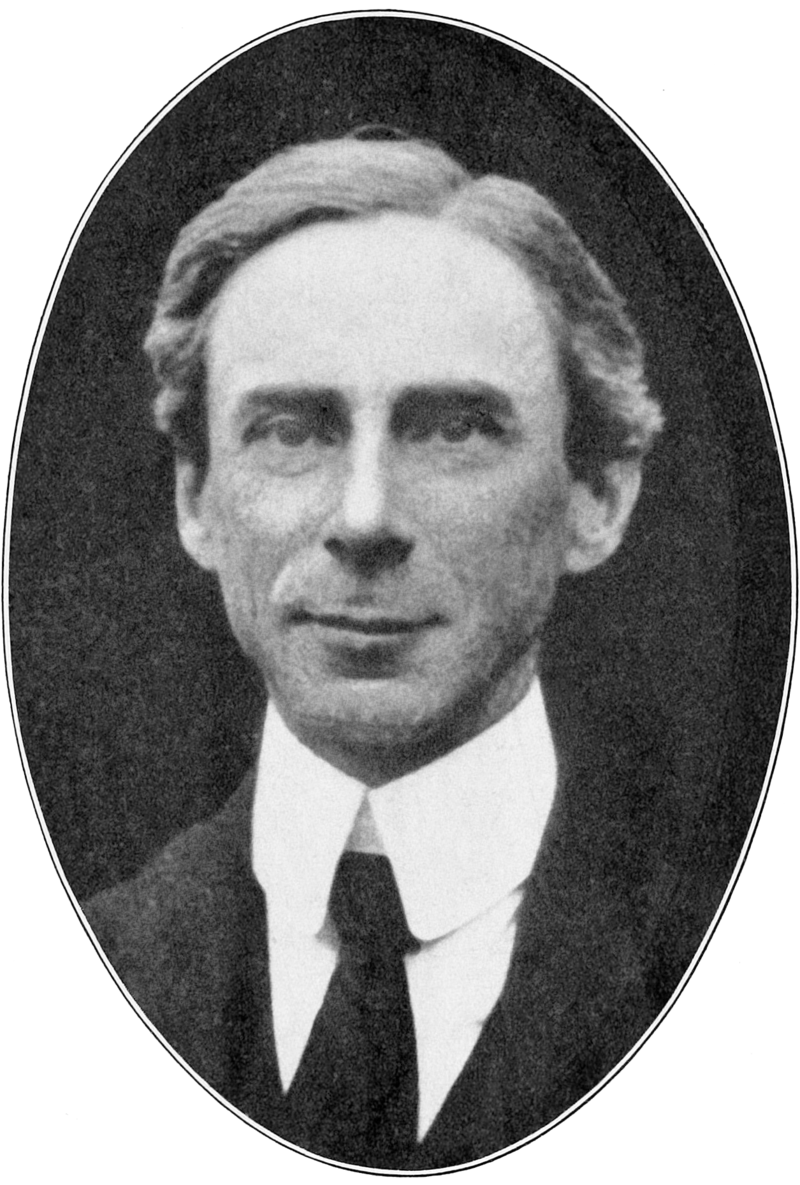
\includegraphics[width=1\textwidth]{800px-Bertrand_Russell_transparent_bg.png}\\
 				\centering
 				Bertrand~Russell \\(1872--1970)
 			\end{minipage}
 		\end{subfigure}
 	\end{figure}
 \end{frame}

 \begin{frame}{Некоторые известные языки и исчисления из математической логики}
 	\begin{itemize}
 		\item Нулевого порядка (высказываний)
 		\item Первого порядка (предикатов)
 		\item Высших порядков
 		\item Исчисление конструкций (calculus of constructions)
 	\end{itemize}
 	\begin{block}{Важное замечание}
 		То, что нельзя записать в языке, нельзя использовать в исчислениях/доказательствах
 	\end{block}
 \end{frame}

 \begin{frame}{Пример: яызк 0го порядка (высказываний) }
 	\frametitle{Знакомая вам булева (бинарная) логика}
 	\begin{figure}[t]
 		\begin{subfigure}[t]{0.45\textwidth}
 			\begin{enumerate}
 				\item Логические константы True и False
 				\item Логические переменные $x,y,z,\dots$
 				\item Бинарные связки $\vee, \wedge, \Rightarrow$ и т.д.
 			\end{enumerate}
 			\vspace{2em}
 			Правила вывода в исчислении, например:
 			\begin{mathpar}
 				\inferrule* [Right=modus ponens]
 				{ P\Rightarrow Q \\    P  }{Q}
 			\end{mathpar}
 		\end{subfigure}
 		\hspace{0.05\textwidth}
 		\begin{subfigure}[t]{0.46\textwidth}
 			\begin{theorem}[Язык и исчисление \textbf{``хорошие''}]
 				Верную формулу можно доказать за конечное число шагов. Ложную можно опровергнуть.\\

 				Т.е. существует алгоритм, который всегда завершается и говорит да/нет.
 			\end{theorem}
 			\vspace{2em}
 			Язык и исчисление \textbf{``плохие''}, потому что не всё можно записать (где кванторы?)
 		\end{subfigure}
 	\end{figure}


 \end{frame}


 \begin{frame}{Разрешимые и неразрешимые задачи}
 	\begin{definition}[Алгоритмически неразрешимая задача]
 		Задача, которая имеет ответ ``да'' или ``нет'', но для которое невозможно реализовать алгоритм, который \emph{всегда завершается, и выдает правильный ответ}.
 	\end{definition}
 	\begin{definition}[Полуразрешимая задача]
 		Неразрешимая задача, для которой можно предъявить алгоритм, который либо дает правильный ответ  ``да'', либо не завершается. Полуразрешимые$^{+}$ умеют говорить ``да'', полуразрешимые$^{-}$ --- ``нет''.
 	\end{definition}
 	Как доказывать неразрешимость
 	\begin{itemize}
 		\item Разбирать случаи и искать противоречие в каждом
 		\item Сводить каноничную неразрешимую задачу к нашей
 	\end{itemize}
 \end{frame}

 \begin{frame}{Язык и исчисление 1-го порядка (предикатов)}
 	%\framesubtitle{Вы это видели на матане}
 	\begin{figure}[t]
 		\begin{subfigure}[t]{0.5\textwidth}
 			Термы:
 			\begin{itemize}
 				\item Предметные константы: 1.0, 42, $\pi$
 				\item Функциональные символы арности  $1\leqslant n$ от термов. Например, $+, \times, f, mod$ и т.д.
 				\item Предметные переменные $x,y,z,\dots$
 			\end{itemize}
 			Формулы:
 			\begin{itemize}
 				\item Логические константы True и False
 				\item Бинарные связки $\vee, \wedge, \Rightarrow$ (и т.д.) %(от двух формул)
 				\item Предикатные символы (от термов) арности $1\leqslant n$
 				\item Кванторы $\forall, \exists$ от имени предметной переменной и формулы
 			\end{itemize}
 		\end{subfigure}
 		\hspace{0.05\textwidth}
 		\begin{subfigure}[t]{0.4\textwidth}
 			\begin{block}{Важно}
 				$+, \times, f, mod$ это названия функциональных символов, никто не гарантирует, что  $+$ это сложение чисел
 			\end{block}
 			\vspace{1em}
 			Пример: \\
 			$\forall x z\ \exists y (x < y) \wedge (y < z)$\\
 			верно, если $x,y,z \in \mathbb{R}$, \\
 			неверно, если $x,y,z \in \mathbb{N}$
 		\end{subfigure}
 	\end{figure}
 \end{frame}

 \begin{frame}{Преимущества и недостатки языка 1го порядка}

 	\begin{itemize}
 		\item Для некоторых формул из синтаксиса можно понять, что они верны (общезначимы). Для них есть алгоритм, который их докажет за конечное число шагов (см. ``метод британского музея'')
 		\item Огромное количество формул верны только в некоторой семантике, для них нельзя предъявить, алгоритм, который завершается и выдает вердикт.\\
 		В общем виде проверка формулы на истинность/ложность -- неразрешимая задача
 		\item Язык недостаточно богат. Кванторы пробегают только предметные переменные, нельзя выразить ``для любой формулы P, верно...'', например, принцип индукции
 		\[
 		\forall P.\quad P(0) \Rightarrow (\forall n . P(n) \Rightarrow P(n+1))  \Rightarrow (\forall n . P(n))
 		\]
 	\end{itemize}
 \end{frame}




 \section{Лямбды как апгрейд языка предикатов}

 \begin{frame}{Но можно попробовать вывернуться}
 	\framesubtitle{Введем специальный синтаксис}

 	\[
 	\lambda P.\quad phormula(P)
 	\]
 	Опишем принцип индукции, и применим его для $P(n)\equiv 0+\dots+n=\frac{n\cdot(n+1)}{2}$
 	\[
 	\lambda P.\quad P(0) \Rightarrow \big{(}\forall n . P(n) \Rightarrow P(n+1)\big{)}  \Rightarrow \big{(}\forall n . P(n)\big{)}
 	\]\pause
 	\[
 	\text{применение/подстановка} \mathlarger{\mathlarger{\mathlarger{\mathlarger{\Downarrow  \quad\!\!\!\!\!\!\Uparrow}}}} \text{абстракция}
 	\]

 	\begin{equation} \label{eq1}
 		\begin{split}
 			(0\equiv0) & \Rightarrow (\forall n . (0+\dots+n=\frac{n\cdot(n+1)}{2}) \Rightarrow \Big{(}0+\dots+(n+1)=\frac{(n+1)\cdot(n+2)}{2}\Big{)})  \\
 			& \Rightarrow (\forall n . 0+\dots+n=\frac{n\cdot(n+1)}{2})
 		\end{split}
 	\end{equation}
 \end{frame}



 \begin{frame}{Правила работы с новым языком $\lambda$}
 	\begin{block}{$\alpha$-эквивалентность}
 		При выборе новых имен, они не должны случайно перекрыть старые.\\
 		Предложения языка, отличающиеся только переименованием переменных, считаются ($\alpha$)эквивалентными
 	\end{block}
 	Например:  если ни $P$, ни $Q$ не встречаются в $phormula$, то $\lambda P. phormula(P)  \alphaequiv{} \lambda Q. phormula(Q) $

 	\begin{block}{$\beta$-эквивалентность}
 		Если у нас встречается $(\lambda P. phormula(P))X$, то мы можем продолжить с этим работать совершив подстановку $X$ вместо $P$ в $phormula$ (записывается как $phormula[P\mapsto X]$), т.е. заменив все свободные вхождения $P$ на $X$ внутри $phormula$.
 	\end{block}
 \end{frame}


